\subsubsection{Aim 2: \SpecificAimTwo}

\paragraph{Rationale}

% \begin{wrapfigure}{R}{4.05in}
%  \begin{mdframed}
%  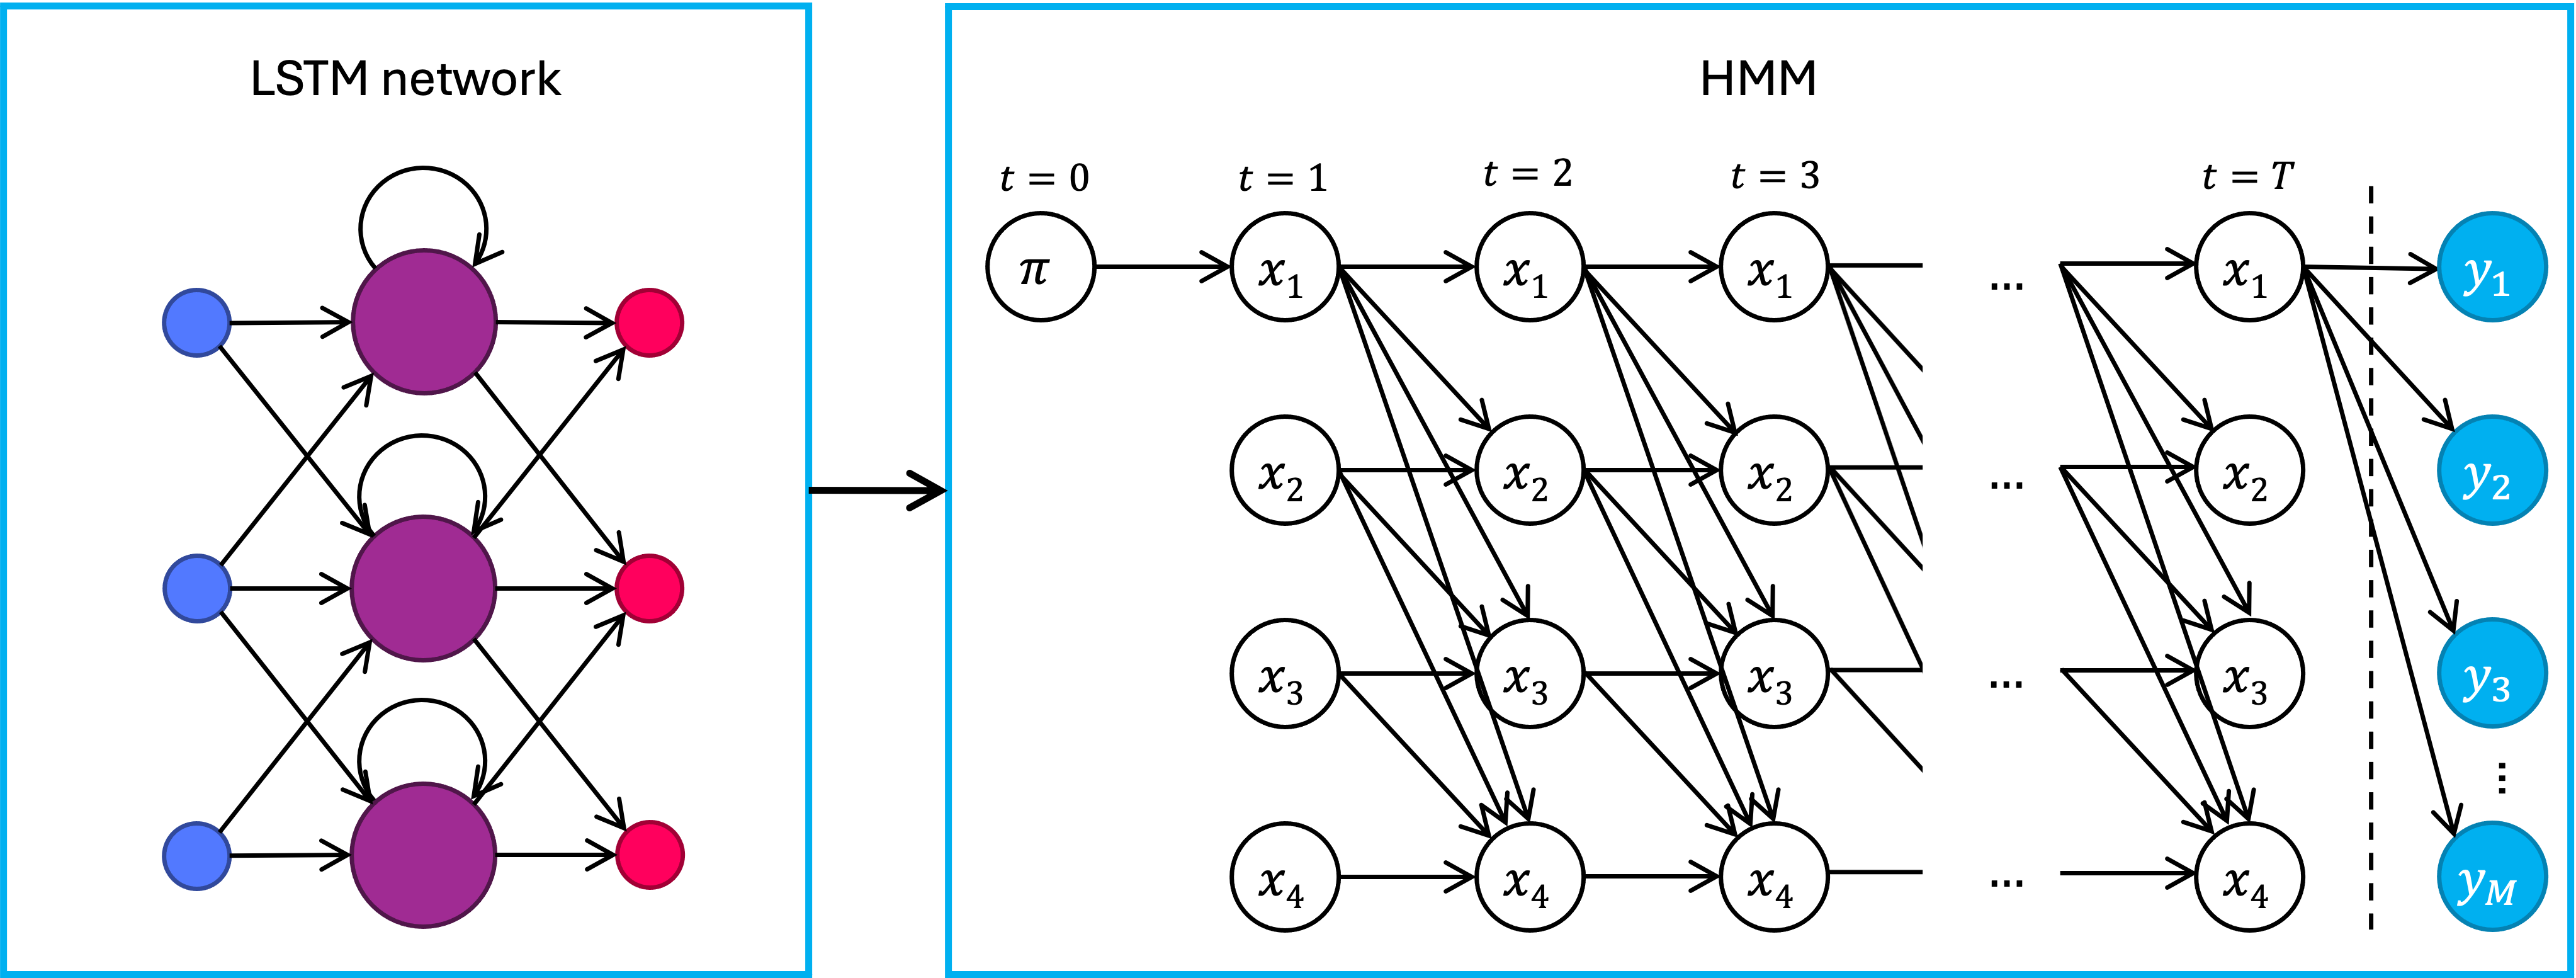
\includegraphics[width=4.0in]{./Figures/LSTM-HMM_diagram.png}
%  \caption{LSTM-HMM architecture. Outputs from the LSTM network are used to inititate the HMM.}
%  \label{LSTM-HMM_diagram}
%  \end{mdframed}
%\end{wrapfigure}

In the realm of cancer research, particularly in studies like those conducted by Gerstung \textit{et al.}, 
traditional methods for modeling mutation timings often rely on statistical models.
These models typically encompass a variety of approaches ranging from regression-based 
frameworks to simpler probabilistic models like Markov chains.
These models are well-established for their interpretability and methodological transparency but 
may lack the nuanced capacity to handle complex, high-dimensional, 
and non-linear patterns that characterize genetic data and cancer progression. % cite?

Unlike conventional statistical models that may not capture complex dependencies, 
the LSTM component of the hybrid model can analyze sequential and temporal data over extended periods. 
This capability allows it to discern underlying patterns that are predictive of 
disease progression that might be overlooked by other methods.
By integrating LSTM-derived insights with an HMM, 
the hybrid model enriches the probabilistic modeling of hidden states. 
The LSTM layer enables the interpretation of details and complexities within 
sequential data that may not be immediately apparent or directly measurable.
Using the LSTM outputs in the HMM model improves the HMM's ability to predict state transitions 
and better capture the complex interactions in the mutation processes.

Utilizing an LSTM enables the model to learn from and adapt to new data dynamically, 
a significant advantage over traditional models that may require static reconfiguration or retraining. 
The integration of LSTM with HMM not only enhances accuracy but also provides finer resolution in the timing of mutations, 
offering detailed insights that are crucial for effective treatment planning and personalized medicine.

\paragraph{2.1. \SpecificAimTwoA}

To harness the predictive power of advanced machine learning for understanding disease progression, 
we propose developing an LSTM network specifically designed to analyze biological sequences. 
The LSTM layer will extract temporal features and patterns that indicate shifts in disease progression. 
The LSTM will output detailed state prediction probabilities and feature vectors that 
encapsulate the dynamic characteristics of the disease, 
providing a rich dataset that reflects both the current state and the likely future states of the disease. 
These outputs from the LSTM will then be fed into the HMM. 
Specifically, the state prediction probabilities generated by the LSTM will be used as emission probabilities in the HMM. 
This step is expected to refine the HMM's ability to map observed data to the correct hidden states. 
Additionally, the feature vectors derived from the LSTM will serve as observations in the HMM. 
This integration enhances the HMM’s capability to accurately model transitions between different disease states, 
leveraging the detailed context provided by the LSTM to improve both the accuracy and reliability of the disease progression model.


\paragraph{2.2. \SpecificAimTwoB}

In this aim, we will implement and optimize both LSTM and HMM models within a unified framework, 
to ensure robust predictions of mutation events. 
To achieve this, we will initially pre-train the LSTM on a designated subset of the PCAWG dataset. 
This preliminary step is designed to stabilize the LSTM's feature extraction capabilities before it is fully integrated with the HMM. 
After we train the LSTM, we will use the outputs of the LTSM to dynamically adjust the parameters of the HMM. 
This adjustment process will utilize a combined training approach that integrates backpropagation for optimizing 
the LSTM alongside the Baum-Welch algorithm for refining the HMM. 
To validate the model's robustness, we will perform cross-validation to prevent overfitting 
and to ensure that the model generalizes effectively across different subsets of data. 
Lastly, we will continuously optimize the model parameters, focusing on improving key performance metrics such as 
accuracy, sensitivity, and specificity in predicting mutation timing. 
This thorough approach to training and validation aims to create a predictive model that is both precise and reliable in its application to real-world clinical data.

%\paragraph{2.3. \SpecificAimTwoC}
%
%Our objective is to apply the fully integrated LSTM-HMM model to the entire NSCLC dataset to assess improvements 
%in the accuracy of mutation timing and to uncover hidden evolutionary patterns. 
%By applying this hybrid model, we aim to focus on achieving detailed and high-resolution timing of mutation events, 
%which is critical for advancing our understanding of cancer progression. 
%Once applied, we will conduct a comparative analysis to juxtapose the mutation timings and evolutionary patterns derived 
%from our hybrid model against those obtained using the traditional Gerstung et al. method. 
%This comparison will not only highlight the differences and improvements brought about by our model 
%but also allow us to evaluate the added value of integrating LSTM with HMM. 
%Specifically, we will assess enhancements in resolution, adaptability, and predictive accuracy, 
%thereby demonstrating the hybrid model's potential to significantly advance the field of cancer genomics.

\paragraph{Challenges \& Alternative Approaches}

In our approach to model complexity and data sparsity, it's important to note that HMMs are inherently proficient at handling sparse data, 
providing a robust fallback mechanism when large datasets are not available. 
This capability allows us to potentially minimize the reliance on extensive machine learning processes in scenarios where data is limited, 
while still maintaining the flexibility to fully leverage more complex machine learning techniques, 
such as those involving LSTM networks, as richer datasets become available. 
By designing the system with this dual capability, we ensure that the model remains effective under varied data conditions,
offering both simplicity and adaptability. 
This approach not only safeguards against overfitting but also ensures that the model can dynamically scale its complexity 
based on the volume and detail of the data it processes.
%